\section[1977年高考数学试卷及答案(天津卷)理科]{1977年普通高等学校招生考试(天津卷)\\\Huge 数学试卷}

\begin{questions}
	\question
	\begin{parts}
		\part 在什么条件下,$\dfrac{y}{2x}$
			\begin{cenum}
				\item 是正数;
				\item 是负数;
				\item 等于零;
				\item 没有意义?
			\end{cenum}

			\begin{solution}
				\begin{cenum}
					\item $\sgn(x)=\sgn(y)$且$x\neq 0$;
					\item $\sgn(x)\neq\sgn(y)$且$x\neq 0$;
					\item $y=0$且$x\neq 0$;
					\item $x=0$
				\end{cenum}
			\end{solution}

		\part 比较下列各组数的大小,并说明理由.
			\begin{cenum}
				\item $\cos\ang{31}$与$\cos\ang{30}$.
				      \begin{solution}
					      \begin{center}
						      \begin{tikzpicture}
							      \begin{axis}[
									      xmin = -pi/2, xmax = 2.5*pi,
									      ymin = -1.5, ymax = 1.5,
								      ]
								      \addplot[domain=0:2*pi]{cos(deg(x))};
								      \addlegendentry{$\cos(x)$}

								      \node[above] at ({pi/2},0) {$\frac{\pi}{2}$};
							      \end{axis}
						      \end{tikzpicture}
					      \end{center}
					      可以看到余弦函数在第一象限是单调递减的,所以$\cos\ang{31} < \cos\ang{30}$.

				      \end{solution}
				\item $\log_21$与$\log_2\frac14$.
				      \begin{solution}
					      对二者分别求值:
					      \begin{align*}
						      \log_21 = \log_2{2^0} = 0 \\
						      \log_2{\frac14} = \log_2{2^{-2}} = -2
					      \end{align*}
					      所以有$\log_21 > \log_2{\frac14}$.
				      \end{solution}
			\end{cenum}
		\part 求值:
			\begin{cenum}
				\item $\tan \left( 5\arcsin\frac{\sqrt{3}}{2} \right)$.
				      \begin{solution}
					      \begin{align*}
						       & = \tan \left( 5\times \frac{\pi}{3} \right) \\
						       & = \tan \left( \frac{5\pi}{3} \right)        \\
						       & = -\sqrt{3}
					      \end{align*}
				      \end{solution}
				\item $(-2)^0 \times (0.01)^\frac12$.
				      \begin{solution}
					      \begin{align*}
						       & = 1 \times 1^{-2\times\frac12} \\
						       & = 1
					      \end{align*}
				      \end{solution}
			\end{cenum}
		\part 计算:$\lg12.5-\lg\frac58+\lg\sin\ang{30}$.
			\begin{solution}
				\begin{align*}
					 & = \lg\frac{25}{2} - \lg\frac58 + \lg\frac12               \\
					 & = \lg \left( \frac{25}{2}\cdot\frac85\cdot\frac12 \right) \\
					 & = \lg10                                                   \\
					 & = 1
				\end{align*}
			\end{solution}

		\part 解方程:
			\begin{math}
				\frac{4x}{x^2-4} - \frac2{x-2} = 1 - \frac1{x+2}.
			\end{math}

			\begin{solution}
				两边同乘以$x^2 - 4, (x\neq\pm2)$得:
				\begin{equation*}
					4x - 2(x+2) = x^2 - 4 - (x-2)
				\end{equation*}
				整理得:
				\begin{equation*}
					x^2 -3x + 2 = 0
				\end{equation*}
				分解因式得:
				\begin{equation*}
					(x-2)(x-1) = 0
				\end{equation*}
				因为$x\neq\pm2$,所以$x=1$.
			\end{solution}

	\end{parts}

	\question
	\begin{parts}
		\part
			某工厂准备在仓库的一侧建立一个矩形储料场(如图),现有$50$米长的铁丝网,如果用它来围成这个储料场,那么长和宽各是多少时,这个储料场的面积最大?并求出这个最大的面积.
			\begin{center}
				\begin{tikzpicture}
					\draw[very thick](0,1) -| (1,.2) (0,-1) -| (1,-.2);
					\draw[thin](1,.7) -| (3, -.7) -- (1,-.7);

					\node at (.5,0){仓库};
					\node at (2,0){储料场};
					\node at (2, -1) {$x$};
					\node[right] at (3, 0) {$y$};
				\end{tikzpicture}
			\end{center}

			\begin{solution}
				面积可以表示成:
				\begin{align*}
					S & = xy          \\
					  & = x(50-2x)    \\
					  & = -2x^2 + 50x
				\end{align*}
				根据抛物线的性质,在$-\frac{b}{2a}=\frac{25}{2}$处面积有最大值,代入面积公式得:
				\begin{equation*}
					S_{max} = \frac{25}{2}(50 - 2\times\frac{25}2) = \qty{312.5}{\meter\squared}
				\end{equation*}
			\end{solution}

		\part 如图,已知$AB$、$DE$是圆$O$的直径,$AC$是弦,$AC\parallel DE$,求证:$CE=EB$.
			\begin{center}
				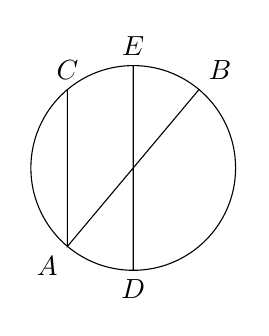
\begin{tikzpicture}[scale=1.3]
					\draw (0,0) circle (1);
					\draw (0,1) -- (0,-1) (50:1) -- (230:1) -- (130:1);

					\node[above] at (0,1) {$E$};
					\node[below] at (0,-1) {$D$};
					\node[above right] at (50:1) {$B$};
					\node[below left] at (230:1) {$A$};
					\node[above] at (130:1) {$C$};
				\end{tikzpicture}
			\end{center}

			\begin{proofsolution}
				\begin{center}
					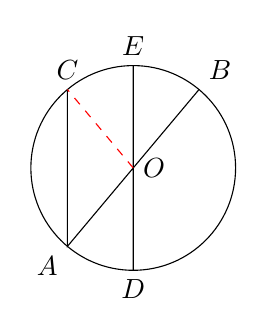
\begin{tikzpicture}[scale=1.3]
						\draw (0,0) circle (1);
						\draw (0,1) -- (0,-1) (50:1) -- (230:1) -- (130:1);

						\node[above] at (0,1) {$E$};
						\node[below] at (0,-1) {$D$};
						\node[above right] at (50:1) {$B$};
						\node[below left] at (230:1) {$A$};
						\node[above] at (130:1) {$C$};

						\draw[dashed, red](0,0) -- (130:1);
						\node[right] at (0,0) {$O$};
					\end{tikzpicture}
				\end{center}
				\begin{cenum}
					\item 连接圆心$O$和$C$点;
					\item
					      \begin{align*}
						       & \because CO = AO                                                 \\
						       & \therefore \angle{A} = \angle{C}                                 \\
						       & \because AC \parallel ED                                         \\
						       & \therefore \angle{C} = \angle{COE} \land \angle{A} = \angle{EOB} \\
						       & \therefore \angle{COE} = \angle{EOB}                             \\
						       & \therefore CE = EB
					      \end{align*}
				\end{cenum}
			\end{proofsolution}
	\end{parts}

	\question 如果已知$bx^2 - 4bx + 2(a+c) = 0\quad (b\neq0)$有两个相等的实数根,求证:$a,b,c$成等差数列.
	\begin{proofsolution}
		因为方程有两个相等的实数根,所以其判别式$\Delta=0$:
		\begin{align*}
			\Delta  = \sqrt{16b^2 - 4b\cdot2(a+c)} = 0 \\
			16b^2 - 8b(a+c) = 0                        \\
			2b = a+ c                                  \\
			b - a = c - b
		\end{align*}
		所以$a,b,c$成等差数列.
	\end{proofsolution}
\end{questions}
